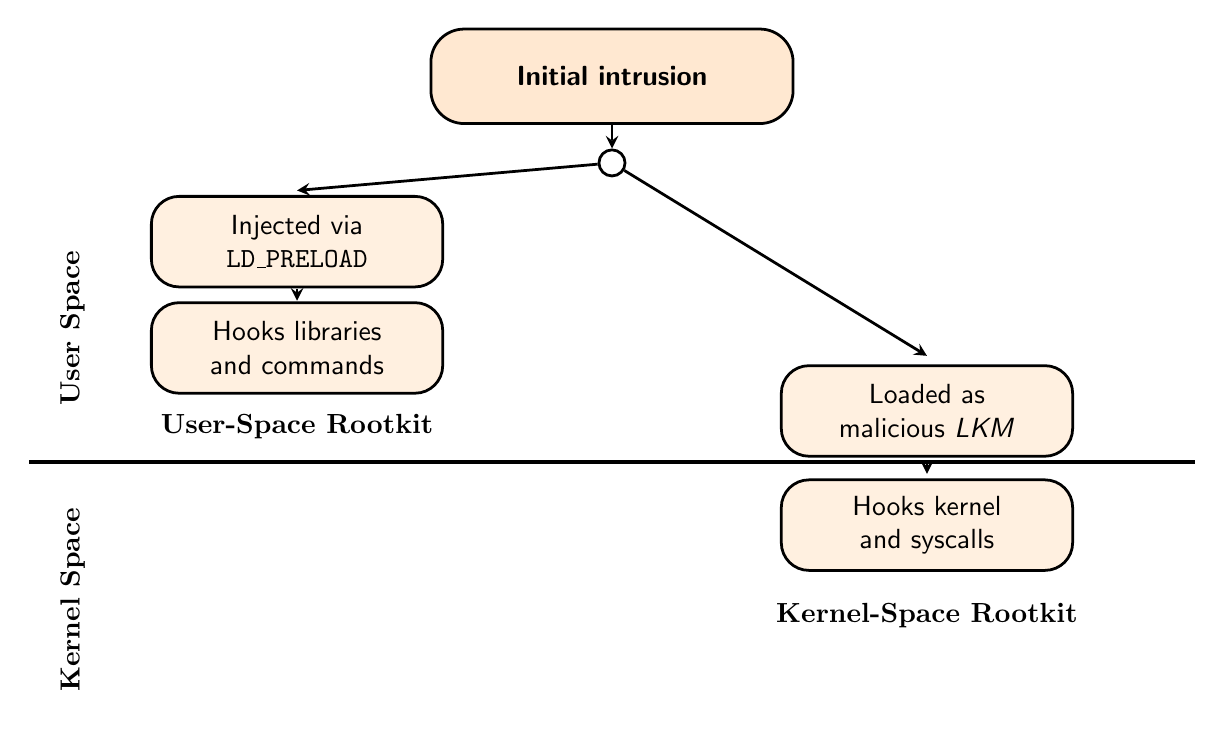
\begin{tikzpicture}[
    font=\sffamily,
    >=stealth,
    box/.style={
        draw=black,
        rounded corners=10pt,
        line width=1pt,
        align=center,
        minimum width=3.7cm,
        minimum height=1.15cm,
        fill=orange!12
    },
    boxdark/.style={
        draw=black,
        rounded corners=10pt,
        line width=1pt,
        align=center,
        minimum width=3.9cm,
        minimum height=1.15cm,
        fill=orange!28
    },
    titlebox/.style={
        draw=black,
        rounded corners=12pt,
        line width=1pt,
        align=center,
        minimum width=4.6cm,
        minimum height=1.2cm,
        fill=orange!18
    }
]

\node[titlebox] (entry) at (0,4.1) {\bfseries Initial intrusion};
\node[circle, draw=black, line width=1pt, fill=white, minimum size=0.18cm] (split) at (0,3.0) {};

\node[box] (u1) at (-4.0,2.0) {Injected via\\\texttt{LD\_PRELOAD}};
\node[box] (u2) at (-4.0,0.65) {Hooks libraries\\and commands};

\node[box] (k1) at (4.0,-0.15) {Loaded as\\malicious \textit{LKM}};
\node[box] (k2) at (4.0,-1.6) {Hooks kernel\\and syscalls};

\draw[line width=1.2pt] (-7.4,-0.8) -- (7.4,-0.8);
\node[rotate=90, font=\bfseries] at (-6.85,0.9) {User Space};
\node[rotate=90, font=\bfseries] at (-6.85,-2.55) {Kernel Space};

\draw[->, line width=1pt] (entry) -- (split);

\draw[->, line width=1pt] (split) -- (-4.0,2.65);
\draw[->, line width=1pt] (-4.0,1.4) -- (-4.0,1.25);

\draw[->, line width=1pt] (split) -- (4.0,0.55);
\draw[->, line width=1pt] (4.0,-0.8) -- (4.0,-0.95);
\node[font=\bfseries] at (-4.0,-0.35) {User-Space Rootkit};
\node[font=\bfseries] at (4.0,-2.75) {Kernel-Space Rootkit};

\end{tikzpicture}
